\documentclass[tikz,border=8pt]{standalone}
\usepackage{tikz}

\begin{document}
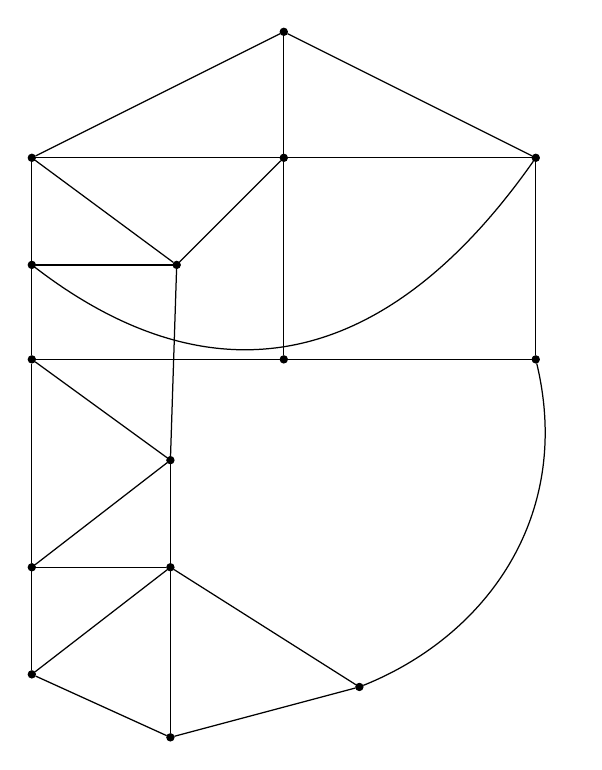
\begin{tikzpicture}[x=0.8cm,y=0.8cm]
  \tikzset{graphvertex/.style={circle,fill=black,draw=black,inner sep=0pt,minimum size=2.6pt}}
  \tikzset{graphedge/.style={draw=black,line width=0.45pt}}

  \node[graphvertex] (v0)  at (0.0, 5.8) {};
  \node[graphvertex] (v1)  at (-4.0, 3.8) {};
  \node[graphvertex] (v2)  at (0.0, 3.8) {};
  \node[graphvertex] (v3)  at (4.0, 3.8) {};
  \node[graphvertex] (v4)  at (-1.7, 2.1) {};
  \node[graphvertex] (v5)  at (-4.0, 2.1) {};
  \node[graphvertex] (v6)  at (0.0, 0.6) {};
  \node[graphvertex] (v7)  at (-4.0, 0.6) {};
  \node[graphvertex] (v8)  at (4.0, 0.6) {};
  \node[graphvertex] (v9)  at (-1.8, -1.0) {};
  \node[graphvertex] (v10) at (-4.0, -2.7) {};
  \node[graphvertex] (v11) at (-1.8, -2.7) {};
  \node[graphvertex] (v12) at (-4.0, -4.4) {};
  \node[graphvertex] (v13) at (-1.8, -5.4) {};
  \node[graphvertex] (v14) at (1.2, -4.6) {};

  \draw[graphedge] (v0) -- (v1);
  \draw[graphedge] (v0) -- (v2);
  \draw[graphedge] (v0) -- (v3);
  \draw[graphedge] (v1) -- (v2);
  \draw[graphedge] (v2) -- (v3);
  \draw[graphedge] (v2) -- (v4);
  \draw[graphedge] (v4) -- (v1);
  \draw[graphedge] (v1) -- (v5);
  \draw[graphedge] (v4) -- (v5);
  \draw[graphedge] (v5) .. controls (-1.4, 0.1) and (1.4, 0.1) .. (v3);

  \draw[graphedge] (v6) -- (v7);
  \draw[graphedge] (v6) -- (v8);
  \draw[graphedge] (v0) -- (v6);
  \draw[graphedge] (v5) -- (v7);
  \draw[graphedge] (v3) -- (v8);

  \draw[graphedge] (v4) -- (v9);
  \draw[graphedge] (v9) -- (v7);
  \draw[graphedge] (v7) -- (v10);
  \draw[graphedge] (v9) -- (v10);
  \draw[graphedge] (v9) -- (v11);
  \draw[graphedge] (v11) -- (v10);
  \draw[graphedge] (v10) -- (v12);
  \draw[graphedge] (v11) -- (v12);
  \draw[graphedge] (v12) -- (v13);
  \draw[graphedge] (v11) -- (v13);
  \draw[graphedge] (v13) -- (v14);
  \draw[graphedge] (v11) -- (v14);
  \draw[graphedge] (v14) .. controls (3.2, -3.8) and (4.6, -1.9) .. (v8);
\end{tikzpicture}
\end{document}
